% !TeX root = ../sustechthesis-example.tex

\chapter[离子阱频率锁定]{离子阱频率锁定}

% \textcolor{red}{这部分主要介绍参考文献\cite[]{Johnson_Wong_Campos_Restelli_Landsman_Neyenhuis_Mizrahi_Monroe_2016}}

带电粒子通常由射频(RF)电势控制,其场梯度提供时间平均力,这些力构成了四极质量滤波器、离子质谱仪和射频(Paul)离子阱等应用的基础\cite[]{Dehmelt_1990, Paul_1990}。这些射频电势,通常在 1 kHz 到 100 MHz 的频率处数百或数千个伏特,在真空中驱动高阻抗负载,通常由射频放大器和谐振升压变换器(例如四分之一波或螺旋谐振器)产生\cite[]{Siverns_Simkins_Weidt_Hensinger_2012}。这种电路容易受到放大器增益、变压器的机械振动和系统中的温度漂移的波动的影响。离子阱对这些波动特别敏感,因为射频电势决定了被捕获离子的谐波振荡频率。稳定的阱频率在从量子信息处理\cite[]{Blatt_Wineland_2008, Monroe_Kim_2013}和量子模拟\cite[]{Richerme_Gong_Lee_Senko_Smith_Foss_Feig_Michalakis_Gorshkov_Monroe_2014, Jurcevic_Lanyon_Hauke_Hempel_Zoller_Blatt_Roos_2014}到原子运动的量子态的制备\cite[]{Leibfried_Blatt_Monroe_Wineland_2003}、原子干涉测量\cite[]{Johnson_Neyenhuis_Mizrahi_Wong_Campos_Monroe_2015}、和量子有限计量\cite[]{Chou_Hume_Koelemeij_Wineland_Rosenband_2010}等方面至关重要。


理论上离子阱中影响阱频率的各种因素
在离子阱系统中,阱频率的表达式为:
\begin{align}
    \omega=e\mu V_0/\sqrt{2}m\Omega R^2
\end{align}

这些参数分别是:
\begin{itemize}
    \item $e$: 离子电荷量;
    \item $\mu$: 几何效率因子;
    \item $m$: 粒子质量;
    \item $R$: 电极间距;
    \item $\Omega$: 输入微波信号的频率;
    \item $V_0$: 输入信号的电压;
\end{itemize}


上面的各个参数中$e$,$\mu$,$m$是常数,R在阱几何形状确定的情况下也是常数。因此,关键的参数在于与射频相关的 $\Omega$ 和 $V_0$ 。这其中,当今射频生成器件自身的频率和幅度稳定性是相当高的,可能产生抖动因素的实际上主要是经过谐振腔后的输出幅度。我们使用的螺线管谐振腔$Q$值较高,只要谐振腔的中心透过频率稍微发生偏移,输出幅度就可能发生较大的抖动。因此阱频稳定或者说阱频锁定主要是通过稳定谐振腔输出的射频幅度实现的。

% 物理上离子阱中影响阱频率的各种因素

受环境振动和温度变化影响,谐振腔的几何形状,主要是螺旋线的长度和腔体长度会发生变化,进而导致谐振腔的中心频率发生偏移。从谐振腔的S参数图中可以看出螺线管谐振腔的Q值很大,透过峰较尖锐,即中心频率附近信号透过衰减较大。因此在输入信号频率抖动极小的情况下,受谐振腔中心频率偏移影响,信号的透过幅度将会发生较大的变化。

\section[离子阱频率锁定原理]{离子阱频率锁定原理}

\section[离子阱频率锁定系统搭建]{离子阱频率锁定系统搭建}

由于系统中需要使用放大器,而放大器对不同频率的信号放大效果有所区别。过大的放大信号可能会损坏谐振腔的分压板,因此这里先用DDS的输出和放大器预先对放大器进行标定,结果如图\ref{fig:helical_lock_amplifier}所示。从接种的拟合直线截距上可以看出,信号功率放大器可以对信号放大月32.83dBm。

\begin{figure}
    \centering
    \caption[DDS输出功率和放大器输出功率]{DDS输出功率和放大器输出功率\label{fig:helical_lock_amplifier}}
    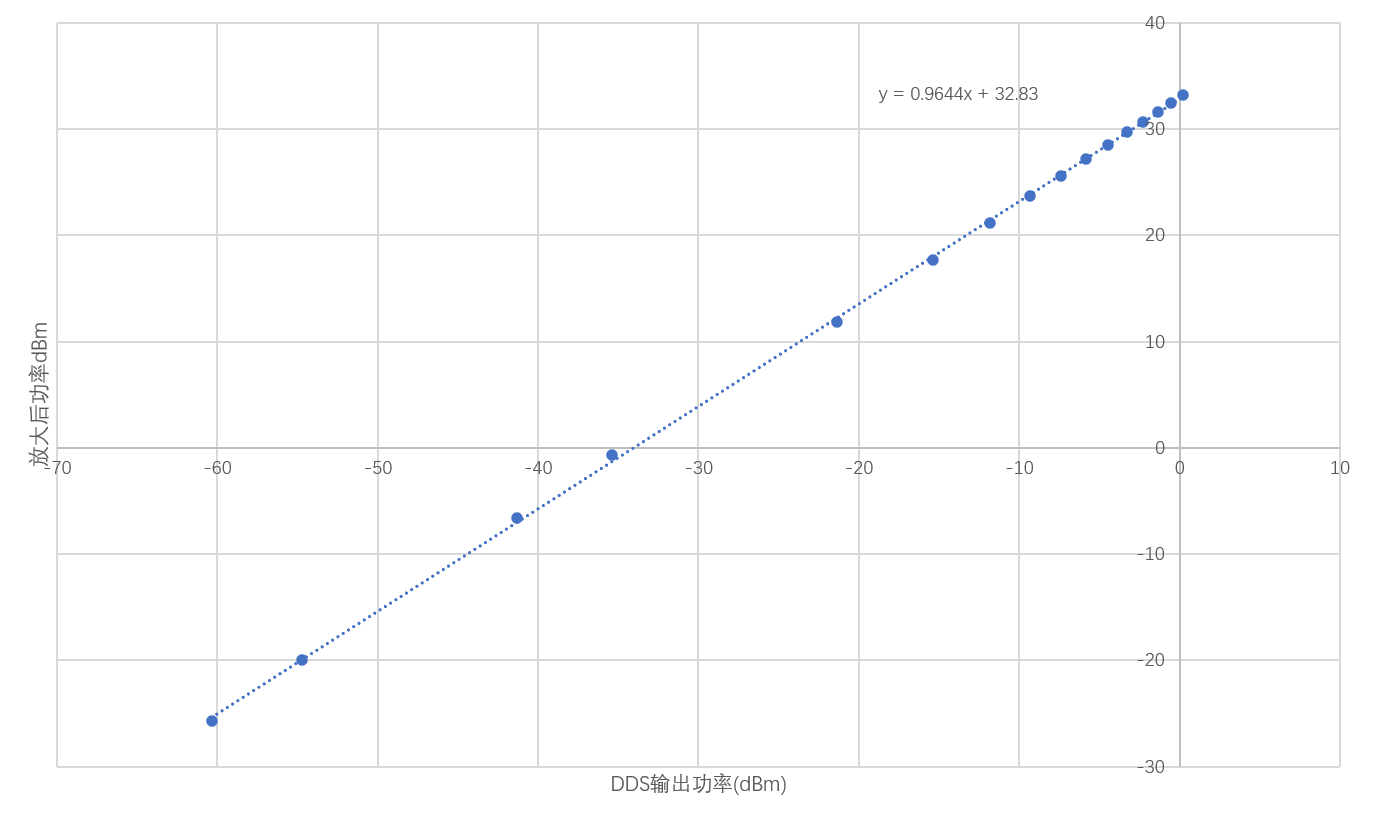
\includegraphics[width=1.0\linewidth]{helical_lock_amplifier}
\end{figure}

阱频锁定模块实验测试图如附录图\ref{fig:trap_frequency_lock_real}所示。

\section[离子阱频率锁定系统结果]{离子阱频率锁定系统结果}


谐振腔输出锁定效果测量结果如图\ref{fig:helical_lock_measure}所示。

\begin{figure}
    \centering
    \caption[谐振腔输出锁定效果测量结果]{谐振腔输出锁定效果测量结果\label{fig:helical_lock_measure}}
    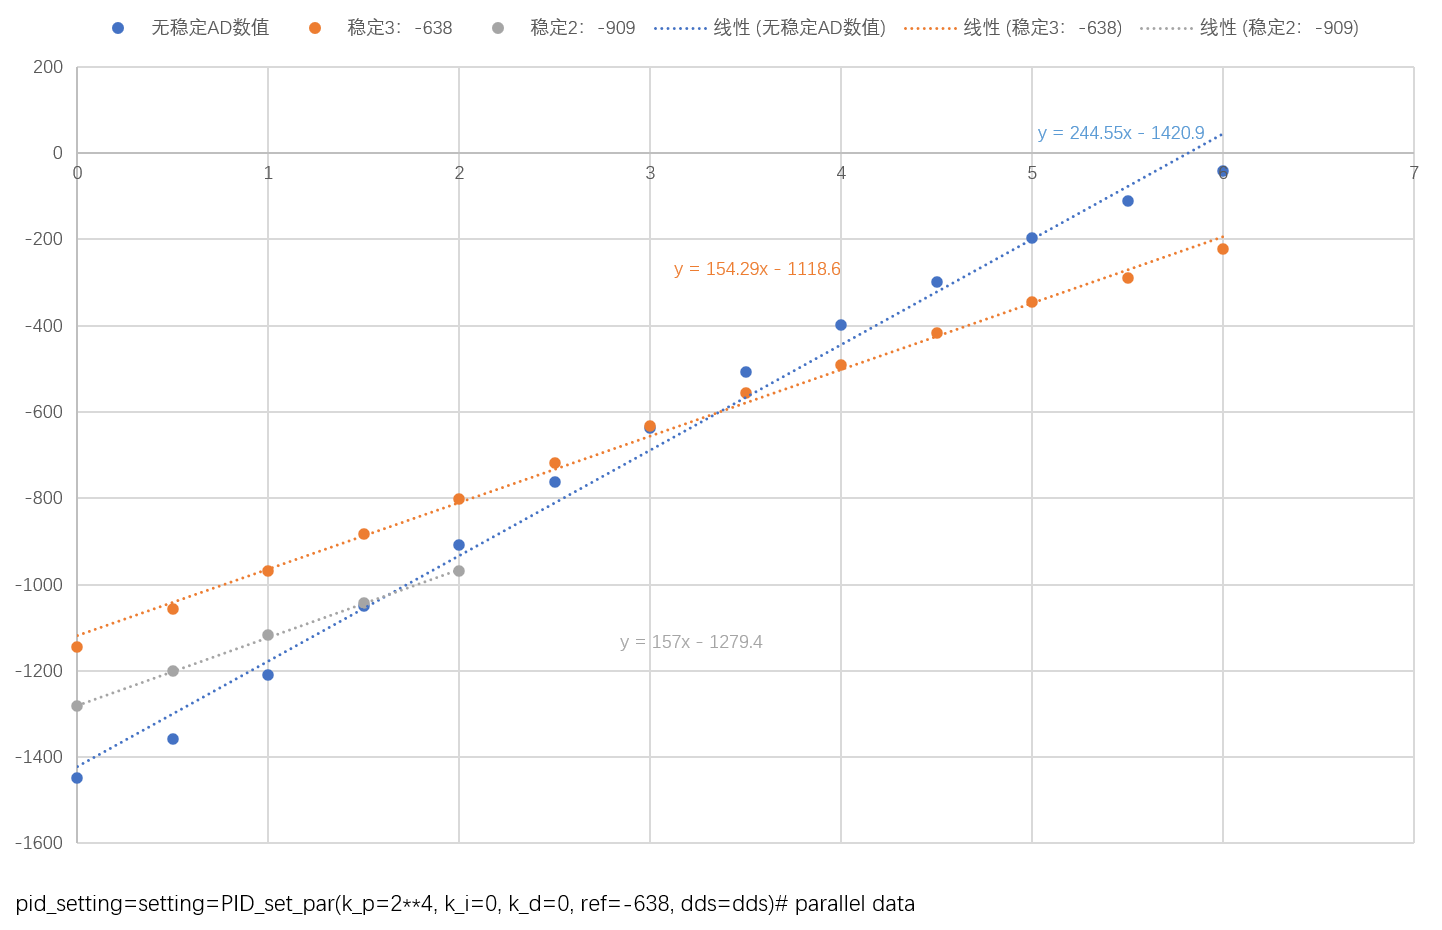
\includegraphics[width=1.0\linewidth]{helical_lock_measure}
\end{figure}


